
\section{Vorlesung}


\subsection{Quantile}
Quartile sind eine Art Quantile. Sie teilen die Anzahl der Werte in gleich große Teile. Quartile teilen mithilfe von 3 Wertegrenzen die Anzahl der Werte in 4 gleichgroße Teile je 25\%.



\subsection{Boxplots}
  \small{\textbf{\textrightarrow (pseudo-) metrisch}}
\vspace{1cm}
  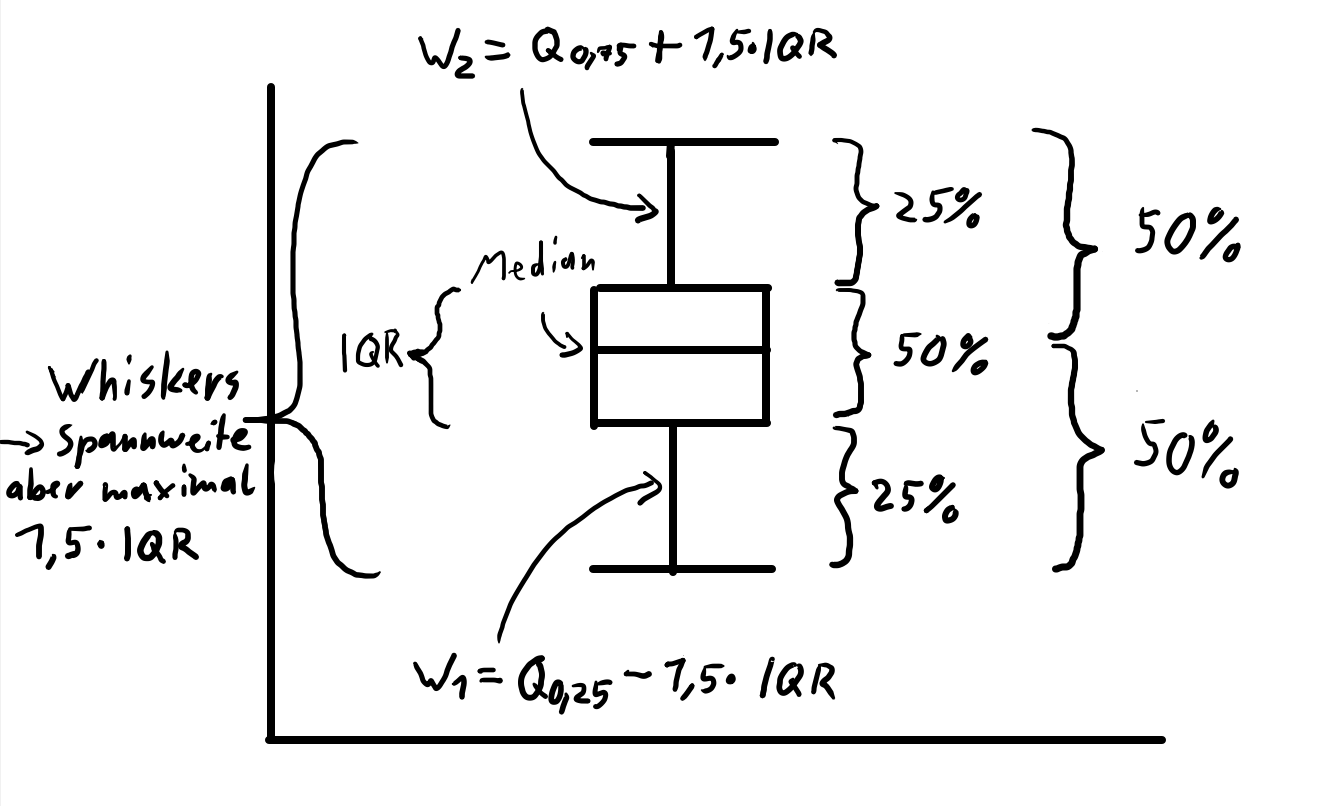
\includegraphics[scale=0.25]{./img/Boxplot.png}

\subsubsection{Ausreißer und Extremwert}
\begin{tabular}{l|l}
  Ausreißer & = \textcolor{red}{1,5~$\cdot$~IQR}~~~über 3. Quartil/ unter 1. Quartil\\
  Extremwert& =\textcolor{red}{~~~~3~$\cdot$~IQR}~~~über 3. Quartil/ unter 1. Quartil
\end{tabular}



\subsection{Variantionskoeffizient V}
  Mit dem Variantionskoeffizienten kann man \textbf{Streuungen} verschiedener Verteilungen vergleichen.
\begin{align*}
  \textrm{V} = \frac{\sigma}{\overline{x}} = \frac{\textrm{Standardabweichung}}{\textrm{arithm. Mittel}} && ;\overline{x}\neq 0
\end{align*}

\subsection{Z-Transformation oder Z-Wert}
  Mit dem Z-Wert kann man \textbf{Werte} verschiedener Verteilungen vergleichen. (In Statistik 2 wird die Z-Transformation im Zusammenhang mit der Standardnormalverteilung sehr wichtig.\\(\href{https://youtu.be/2tuBREK_mgE?t=163}{Ein interessantes Youtubevideo, es nimmt allerdings schon einige Zusammenhänge vorweg, die später nocheinmal richtig in Statistik 2 vorkommen}))


\begin{align*}
 \textrm{z} &= \frac{x_{\textrm{i}} - \overline{x}}{\sigma}
\end{align*}
- Mittelwert aller Z-Werte = 0\\
- Varianz    aller Z-Werte = 1

\begin{comment}
\subsection{Übung}
\begin{enumerate}
\end{enumerate}
\end{comment}

%Aufgabe zu variantionskoeffizient einfügen
